%
% This document contains the chapter about synthesizing circuits.
%
% Copyright (C) 2005, 2006 Stefan Jahn <stefan@lkcc.org>
% Copyright (C) 2005 Michael Margraf <Michael.Margraf@alumni.TU-Berlin.DE>
%
% Permission is granted to copy, distribute and/or modify this document
% under the terms of the GNU Free Documentation License, Version 1.1
% or any later version published by the Free Software Foundation.
%

\chapter{Synthesizing circuits}
\label{sec:synthesis}

\section{Attenuators}

Attenuators are used to damp a signal. Using pure ohmic resistors
the circuit can be realized for a very high bandwidth, i.e. from
DC to many GHz. The power attenuation $0 < L\le 1$ is defined as:
\begin{equation}
\label{eqn:loss}
L = \dfrac{P_{in}}{P_{out}}
  = \dfrac{V_{in}^2}{Z_{in}}\cdot\dfrac{Z_{out}}{V_{out}^2}
  = \left( \dfrac{V_{in}}{V_{out}}\right)^2 \cdot\dfrac{Z_{out}}{Z_{in}}
\end{equation}
where $P_{in}$ and $P_{out}$ are the input and output power and
$V_{in}$ and $V_{out}$ are the input and output voltages.

\begin{figure}[ht]
\begin{center}
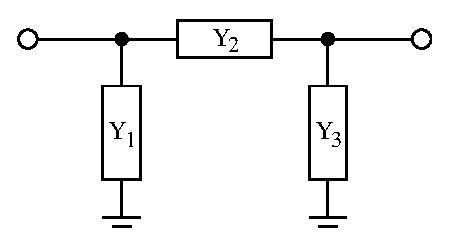
\includegraphics[width=5cm]{picircuit}
\end{center}
\caption{$\pi$-topology of an attenuator}
\label{fig:pi_attenuator}
\end{figure}
\FloatBarrier

Fig. \ref{fig:pi_attenuator} shows an attenuator using the
$\pi$-topology. The conductances can be calculated as follows.
\begin{align}
Y_2 & = \dfrac{L - 1}{2\cdot \sqrt{L\cdot Z_{in}\cdot Z_{out}}} \\
Y_1 & = Y_2\cdot\left( \sqrt{\dfrac{Z_{out}}{Z_{in}}\cdot L} - 1 \right) \\
Y_3 & = Y_2\cdot\left( \sqrt{\dfrac{Z_{in}}{Z_{out}}\cdot L} - 1 \right)
\end{align}
where $Z_{in}$ and $Z_{out}$ are the input and output reference
impedances, respectively. The $\pi$-attenuator can be used for an
impedance ratio of:
\begin{equation}
\dfrac{1}{L} \le \dfrac{Z_{out}}{Z_{in}} \le L
\end{equation}

\begin{figure}[ht]
\begin{center}
\includegraphics[width=5cm]{tcircuit}
\end{center}
\caption{T-topology of an attenuator}
\label{fig:t_attenuator}
\end{figure}
\FloatBarrier

Fig. \ref{fig:t_attenuator} shows an attenuator using the
T-topology. The resistances can be calculated as follows.
\begin{align}
Z_2 & = \dfrac{2\cdot \sqrt{L\cdot Z_{in}\cdot Z_{out}}}{L - 1} \\
Z_1 & = Z_{in}\cdot A - Z_2 \\
Z_3 & = Z_{out}\cdot A - Z_2 \\
\textrm{with} \qquad A & = \dfrac{L + 1}{L - 1}
\end{align}
where $L$ is the attenuation ($0 < L\le 1$) according to
equation \ref{eqn:loss} and $Z_{in}$ and $Z_{out}$
are the input and output reference impedance, respectively.
The T-attenuator can be used for an impedance ratio of:
\begin{equation}
\dfrac{Z_{out}}{Z_{in}} \le \dfrac{(L+1)^2}{4\cdot L}
\end{equation}

\section{Filters}

One of the most common tasks in microwave technologies is to
extract a frequency band from others. Optimized filters exist
in order to easily create a filter with an appropriate characteristic.
The most popular ones are:

\addvspace{12pt}

\begin{tabular}{l|l}
Name & Property \\
\hline
Bessel filter (Thomson filter) & as constant group delay as possible \\
Butterworth filter (power-term filter) & as constant amplitude transfer function as possible \\
Chebychev filter type I & constant ripple in pass band \\
Chebychev filter type II & constant ripple in stop band \\
Cauer filter (elliptical filter) & constant ripple in pass and stop band \\
\end{tabular} 

\addvspace{12pt}

From top to bottom the following properties increase:
\begin{itemize}
\item ringing of step response
\item phase distortion
\item steepness of amplitude transfer function at the beginning of the pass band
\end{itemize}

\addvspace{12pt}

The order $n$ of a filter denotes the number of poles of its (voltage)
transfer function. It is:
\begin{equation}
\text{slope of asymptote} = \pm\, n\cdot 20 \text{dB/decade}
\end{equation}
Note that this equation holds for all filter characteristics, but
there are big differences concerning the attenuation near the pass
band.


\subsection{LC ladder filters}

The best possibility to realize a filters in VHF and UHF bands are
LC ladder filters. The usual way to synthesize them is to first
calculate a low-pass (LP) filter and afterwards transform it into a
high-pass (HP), band-pass (BP) or band-stop (BS) filter. To do so,
each component must be transformed into another.

\addvspace{12pt}

In a low-pass filter, there are  parallel capacitors $C_{LP}$ and
series inductors $L_{LP}$ in alternating order. The other filter
classes can be derived from it:

\addvspace{12pt}

In a high-pass filter:
\begin{align}
C_{LP} \quad \rightarrow \quad & L_{HP} = \dfrac{1}{\omega_B^2\cdot C_{LP}} \\
L_{LP} \quad \rightarrow \quad & C_{HP} = \dfrac{1}{\omega_B^2\cdot L_{LP}}
\end{align}

\addvspace{12pt}

In a band-pass filter:
\begin{align}
C_{LP} \quad \rightarrow \quad & \text{parallel resonance circuit with} \\
                               & C_{BP} = \dfrac{C_{LP}}{\Delta\Omega} \\
                               & L_{BP} = \dfrac{\Delta\Omega}{\omega_1\cdot \omega_2\cdot C_{LP}} \\
L_{LP} \quad \rightarrow \quad & \text{series resonance circuit with} \\
                               & C_{BP} = \dfrac{\Delta\Omega}{\omega_1\cdot \omega_2\cdot L_{LP}} \\
                               & L_{BP} = \dfrac{L_{LP}}{\Delta\Omega}
\end{align}

\addvspace{12pt}

In a band-stop filter:
\begin{align}
C_{LP} \quad \rightarrow \quad & \text{series resonance circuit with} \\
       & C_{BP} = \dfrac{C_{LP}}{2\cdot\left| \dfrac{\omega_2}{\omega_1} - \dfrac{\omega_1}{\omega_2} \right| } \\
       & L_{BP} = \dfrac{1}{\omega^2\cdot \Delta\Omega\cdot C_{LP}} \\
L_{LP} \quad \rightarrow \quad & \text{parallel resonance circuit with} \\
       & C_{BP} = \dfrac{1}{\omega^2\cdot \Delta\Omega\cdot L_{LP}} \\
       & L_{BP} = \dfrac{L_{LP}}{2\cdot\left| \dfrac{\omega_2}{\omega_1} - \dfrac{\omega_1}{\omega_2} \right| }
\end{align}

\addvspace{12pt}

Where
\begin{align}
\omega_1 \quad\rightarrow\quad & \text{lower corner frequency of frequency band} \\
\omega_2 \quad\rightarrow\quad & \text{upper corner frequency of frequency band} \\
\omega   \quad\rightarrow\quad & \text{center frequency of frequency band} \quad \omega = 0.5\cdot (\omega_1 + \omega_2) \\
\Delta\Omega \quad\rightarrow\quad & \Delta\Omega = \dfrac{|\omega_2 - \omega_1|}{\omega}
\end{align}

\subsubsection{Butterworth}

The $k$-th element of an $n$ order Butterworth low-pass ladder filter is:
\begin{alignat}{3}
 & \text{capacitance:} \qquad & C_k = & \dfrac{X_k}{Z_0} \\
 & \text{inductance:}  \qquad & L_k = & X_k \cdot Z_0 \\
 & \text{with}         \qquad & X_k = & \dfrac{2}{\omega_B} \cdot \sin \dfrac{(2\cdot k + 1)\cdot\pi}{2\cdot n}
\end{alignat}

The order of the Butterworth filter is dependent on the specifications
provided by the user.  These specifications include the edge
frequencies and gains.
\begin{equation}
\label{eq:ButtOrder}
n = \dfrac{\log{\left(\dfrac{10^{-0.1\cdot \alpha_{stop}} - 1}{10^{-0.1\cdot \alpha_{pass}} - 1}\right)}}{2\cdot\log{\left(\dfrac{\omega_{stop}}{\omega_{pass}}\right)}}
\end{equation}

\subsubsection{Chebyshev I}

The equations for a Chebyshev type I filter are defined recursivly.
With $R_{dB}$ being the passband ripple in decibel, the $k$-th
element of an $n$ order low-pass ladder filter is:
\begin{alignat}{3}
 & \text{capacitance:} \qquad & C_k & = \dfrac{X_k}{Z_0} \\
 & \text{inductance:}  \qquad & L_k & = X_k \cdot Z_0 \\
 & \text{with}         \qquad & X_k & = \dfrac{2}{\omega_B}\cdot g_k \\
 & & r   & = \sinh\left( \frac{1}{n}\cdot\text{arsinh}\dfrac{1}{\sqrt{10^{R_{dB}/10} - 1}} \right) \\
 & & a_k & = \sin \dfrac{(2\cdot k + 1)\cdot\pi}{2\cdot n} \\
 & & g_k & =
\begin{cases}
\begin{array}{ll}
  \dfrac{a_k}{r} & \textrm{ for } \quad k=0\\
  \dfrac{a_{k-1}\cdot a_k}{g_{k-1}\cdot \left( r^2 + \sin^2\dfrac{k\cdot\pi}{n} \right)} & \textrm{ for } \quad k\ge 1
\end{array}
\end{cases} \\
 & & X_k & = \dfrac{2}{\omega_B}\cdot g_k
\end{alignat}

The order of the Chebychev filter is dependent on the specifications
provided by the user.  The general form of the calculation for the
order is the same as for the Butterworth, except that the inverse
hyperbolic cosine function is used in place of the common logarithm
function.
\begin{equation}
\label{eq:ChebOrder}
n = \dfrac{\textrm{sech}\left(\dfrac{10^{-0.1\cdot \alpha_{stop}} - 1}{10^{-0.1\cdot \alpha_{pass}} - 1}\right)}{2\cdot\textrm{sech}\left(\dfrac{\omega_{stop}}{\omega_{pass}}\right)}
\end{equation}

\subsubsection{Chebyshev II}

Because of the nature of the derivation of the inverse Chebychev approxiation function from the standard Chebychev approximation the calculation of the order \eqref{eq:ChebOrder} is the same.


\section{Matching newtworks}
The matching networks are essential in RF circuit design since they are aimed to maximize the power transfer (i.e. $S_{11} \rightarrow$ 0). They can be implemented using lumped components (more common in RF applications), but also using transmission lines (more common in the microwave band and higher). In what follows, it will be depicted the design equations for the methods included in the matching network tool.
\subsection{LC}
\subsection{Single stub}
Any complex load can be matched using the single stub implementation. The variables are the distance between the stub and the load, and the length of the stub. Let be $Z_L = R_L +jX_L$ the load impedance, then the impedance at the stub is:

\begin{figure}
\centering
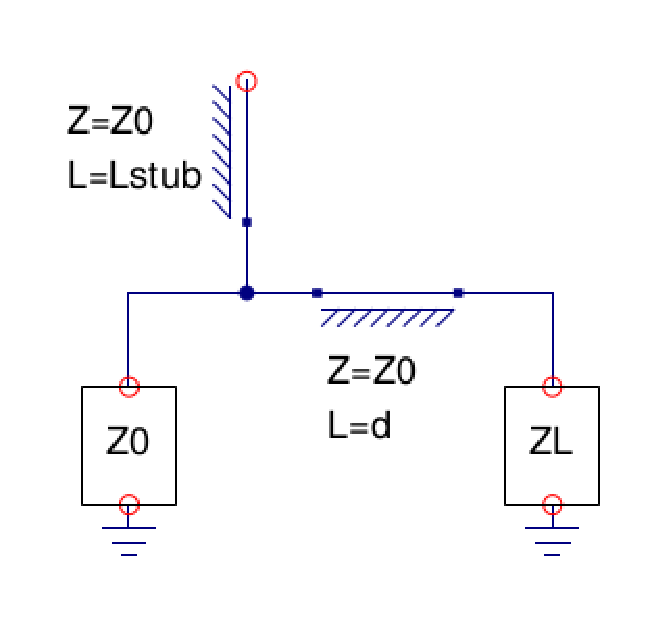
\includegraphics[width=50mm]{SingleStubOpen.eps}
\caption{Single stub matching network. Open circuit configuration}
\end{figure}


\begin{figure}
\centering
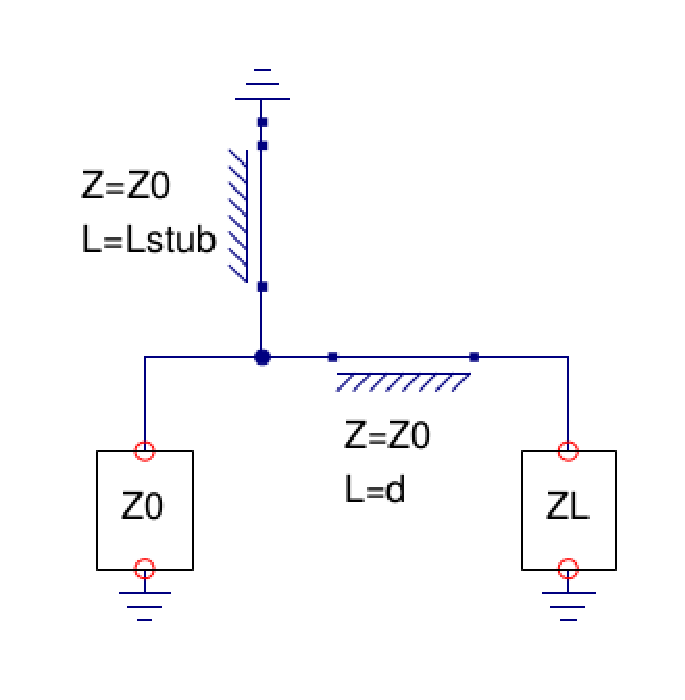
\includegraphics[width=50mm]{SingleStubShort.eps}
\caption{Single stub matching network. Short circuit configuration}
\end{figure}

\begin{equation}
Z(d) = Z_0 \frac{Z_L + j\cdot Z_0\cdot tan(\beta \cdot d)}{Z_0 + j\cdot Z_L \cdot tan(\beta \cdot d)}
\end{equation}

\noindent where $\beta = \frac{2\pi}{\lambda}$ is the wave number and $d$ the distance between the load and the stub. The admitance at the stub is: $Y(d) = G(d)+j \cdot B(d)$, where G(d) is the conductance and B(d) the susceptance at d. It can be shown that:

\begin{equation}
G(d) = \frac{R_L \cdot (1 + tan^2(\beta \cdot d))}{R_L^2 + (X_L + Z_0\cdot tan(\beta \dot d))^2}
\end{equation}

\noindent and, 

\begin{equation}
B(d) = \frac{R_L^2\cdot tan(\beta \cdot d) - (Z_0 - X_L\cdot tan(\beta \cdot d))\cdot (X_L + Z_0\cdot tan(\beta \cdot d))}{Z_0 \cdot (R_L^2 + (X_L + Z_0\cdot tan(\beta \cdot d))^2)}
\end{equation}

The conductance at the stub should be $G(d) = 1/Z_0$ so as to match the real part of the load to $Z_0$. Then, applying this condition and solving the previous equation for $t = tan(\beta \cdot d)$, it gives:

\begin{equation}
t = \frac{X_L \pm \sqrt{(R_L/Z_0) \cdot ((Z_0 - R_L)^2 + X_L^2)}}{R_L - Z_0} \;\;\;\;\; R_L \neq Z_0
\end{equation}

\begin{equation}
t = -X_L/(2\cdot Z_0) \;\;\;\;\; R_L == Z_0
\end{equation}

\noindent Now, the susceptance of the stub should be calculated to cancel the reactive part of the load impedance, so $B_{stub} = -B(d)$.

\noindent Since $t=tan(\beta \cdot d)$, $d$ can be calculated as:

\begin{equation}
d = \frac{\lambda}{2\pi} atan(t) \;\;\;\;\;\;\;\; \text{if t $\geq$ 0}
\end{equation}

\begin{equation}
d = \frac{\lambda}{2\pi} (\pi + atan(t)) \;\;\;\;\;\;\;\; \text{if t $<$ 0}
\end{equation}

\noindent The length of the stub is given by:

\begin{equation}
l_{open} = \frac{-\lambda}{2\pi} atan\left(Z_0\cdot B(d)\right)   \;\;\;\;\;\;\;\; \text{Open stub}
\end{equation}

\begin{equation}
l_{short} = \frac{\lambda}{2\pi} atan\left(\frac{1}{Z_0\cdot B(d)}\right) \;\;\;\;\;\;\;\; \text{Short circuited stub}
\end{equation}

\subsection{Double stub}
The single stub method is really useful since it can match any load. However, the distance between the load and the stub depends on $Z_L$ and this might be a problem for some applications. To overcome this problem, the double stub technique may be used.\\

\begin{figure}
\centering
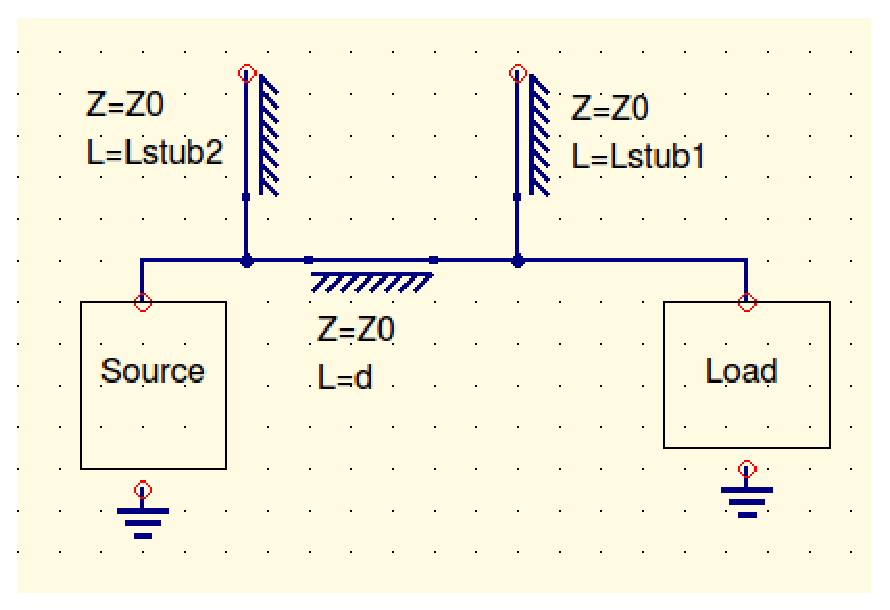
\includegraphics[width=50mm]{DoubleStubOpen.eps}
\caption{Double stub matching network. Open circuit configuration}
\end{figure}


\begin{figure}
\centering
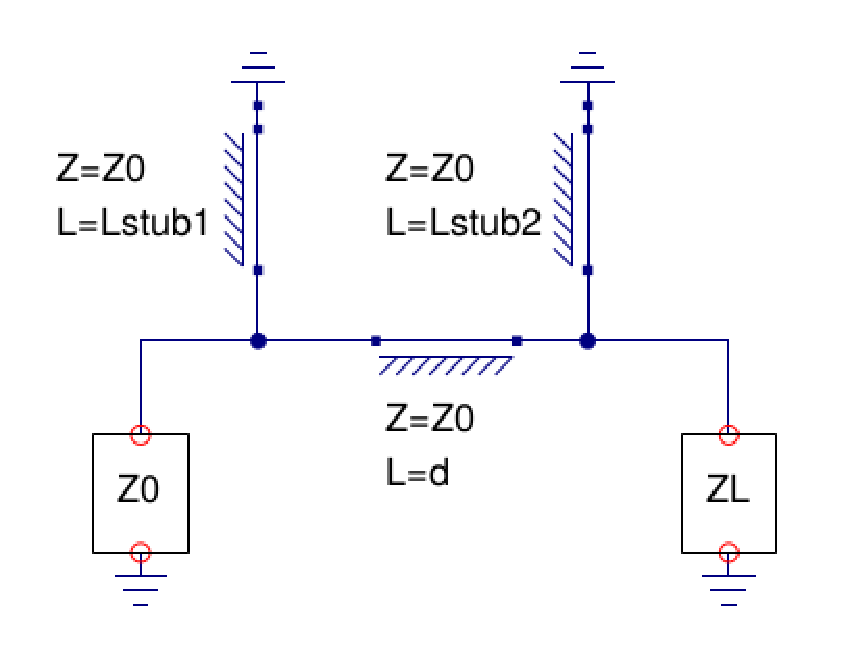
\includegraphics[width=50mm]{DoubleStubShort.eps}
\caption{Double stub matching network. Short circuit configuration}
\end{figure}

The admitance at the first stub is $Y_1 = G_L + j(B_L + B_{stub_1})$, where $Y_L$, $B_L$ and $G_L$ have the same meaning as in the previous section. $B_{stub1}$ is the susceptance of the first stub.

The distance between the stubs, $d$, is typically set to $\lambda/8$ and it is fixed beforehand. Under this condition, the admitance at the second stub is given by:

\begin{equation}
Y_2 = Y_0 \frac{G_L + j(B_L + B_{stub1} + Y_0 \cdot tan(\beta \cdot d))}{Y_0 + j (G_L + j(B_L + B_{stub1})) \cdot tan(\beta \cdot d)}
\end{equation}

Since, the impedance at the second stub must be $Z_0$, so equating $Real\lbrace Y_2 \rbrace = 1/Z_0$ it gives:

\begin{equation} 
G_L = Y_0\frac{1 + tan^2(\beta \cdot d)}{2tan^2(\beta \cdot d)} \lbrace 1 \pm \sqrt{1 - \frac{4tan^2(\beta \cdot d)(Y_0 - (B_L+B_{stub1})\cdot tan(\beta \cdot d))^2}{Y_0^2(1+tan^2(\beta \cdot d))^2}} \rbrace
\end{equation}

Notice that when the factor inside the square root becomes negative, the double stub cannot match the load conductance. Therefore, it can be match load conductances such that:

\begin{equation}
G_L \leq \frac{Y_0}{sin^2(\beta \cdot d)}
\end{equation}

If it is possible to match the conductance of the load, the susceptance of the first stub can be calculated as:
\begin{equation}
B_{stub_1} = - B_L + \frac{Y_0 \pm \sqrt{(1 + tan^2(\beta \cdot d))G_L\cdot Y_0 - (G_L \cdot tan(\beta \cdot d))^2}}{tan(\beta \cdot d)}
\end{equation}


\noindent Similarly, the susceptance of the second stub is:
\begin{equation}
B_{stub_2} = \frac{\pm\sqrt{Y_0\cdot G_L(1 + tan^2(\beta \cdot d)) - (G_L\cdot tan(\beta \cdot d))^2} + G_L \cdot Y_0}{G_L \cdot tan(\beta \cdot d)}
\end{equation}

\noindent Finally, the length of the stubs can be calculated as:

\begin{equation}
l_{open} = \frac{\lambda}{2\pi} atan\left(Z_0\cdot B_{stub_i}\right)   \;\;\;\;\;\;\;\; \text{Open stub}
\end{equation}

\begin{equation}
l_{short} = \frac{-\lambda}{2\pi} atan\left(\frac{1}{Z_0\cdot B_{stub_i}}\right) \;\;\;\;\;\;\;\; \text{Short circuited stub}
\end{equation}

\noindent where $i$ denotes the number of the stub. 

\subsection{Multistage $\lambda$/4 sections}
\subsubsection{Binomial weighting}
\subsubsection{Chebyshev weighting}
